\chapter{Fonctionnement et tests}

Dans cette partie nous chercherons à décrire dans un premier temps les fonctionnements, ou, le cas échéant, les non fonctionnements de notre application.  Nous aborderons ensuite la politique de tests effectuée pour vérifier notre code. 

\section{Fonctionnement}

Lorsque l'on lance l'application, on exécute l'interface graphique. Cette interface fait appel aux auters parties de l'architecture pour afficher et organiser ses composants.

\subsection{Interface Graphique (GUI)}

La méthode \textit{main} de Start.java est appelée lors du démarrage de l'application. Cette méthode fait créé une instance de UserGUI, la première page de l'application qui s'affiche.

\begin{figure}[!ht]
\begin{center}
  \fbox{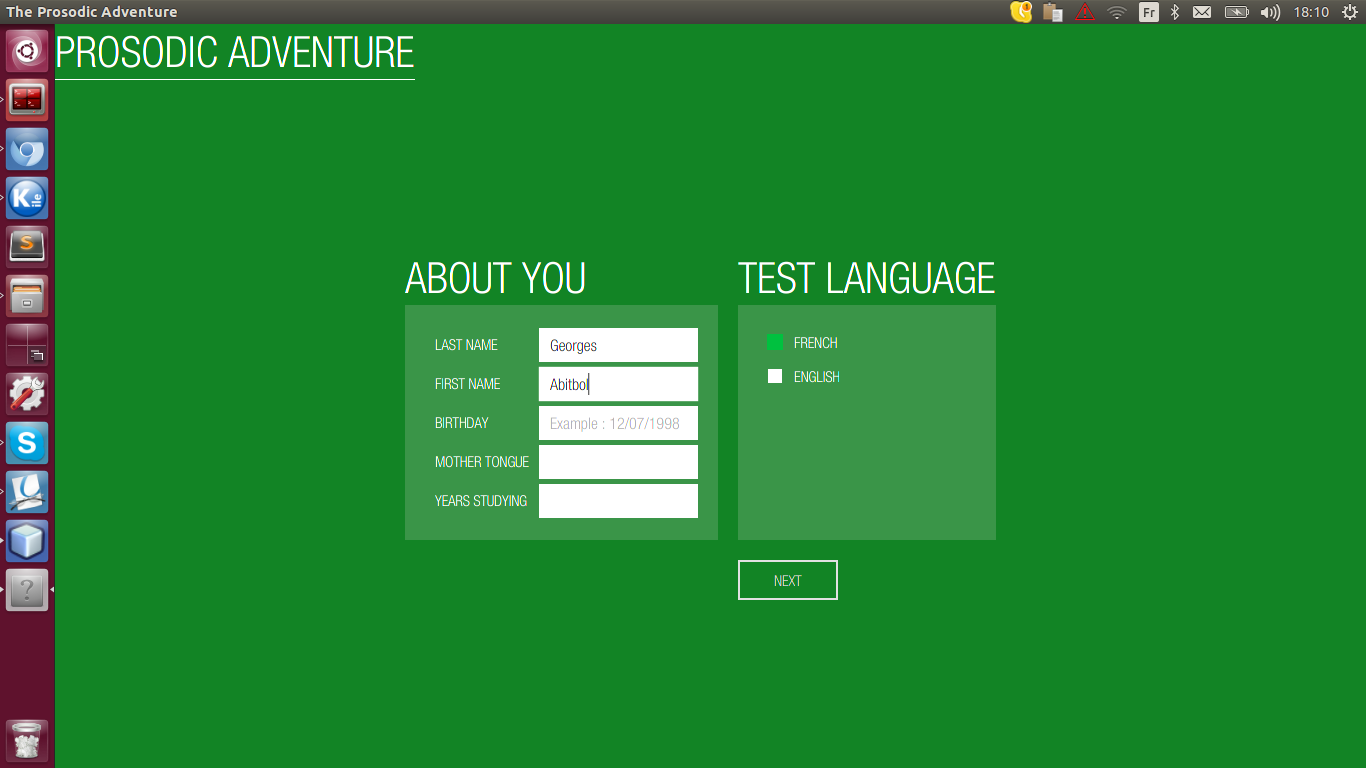
\includegraphics[width=8cm]{./fonctionnement_tests/UserGUI.png}}
  \caption{Fonctionnement - UserGUI}
  \label{UserGUI} 
\end{center}
\end{figure}

Pour récupérer les langues disponibles, UserGUI fait appel au contrôleur, dont nous décrirons le fonctionnement par la suite.
Les informations entrées par l'utilisateur dans les champs de ``\textsc{about you}'' (voir \textsc{Figure} \ref{UserGUI}) sont récupérés lors du clic sur le bouton ``\textsc{next}''. Ces données sont récupérées dans un fichier \textit{txt} par le biais du package \textit{Extract} que nous allons voir plus tard.

Après l'exportation des données sur l'utilisateur, un lien est fait vers la seconde page de l'interface : ChooseGUI (voir \textsc{Figure} \ref{ChooseGUI}). Cette page est une simple page avec deux boutons pour savoir dans quel mode veut aller l'utilisateur (apprentissage da l'application ou test concret).

\newpage

\begin{figure}[!ht]
\begin{center}
  \fbox{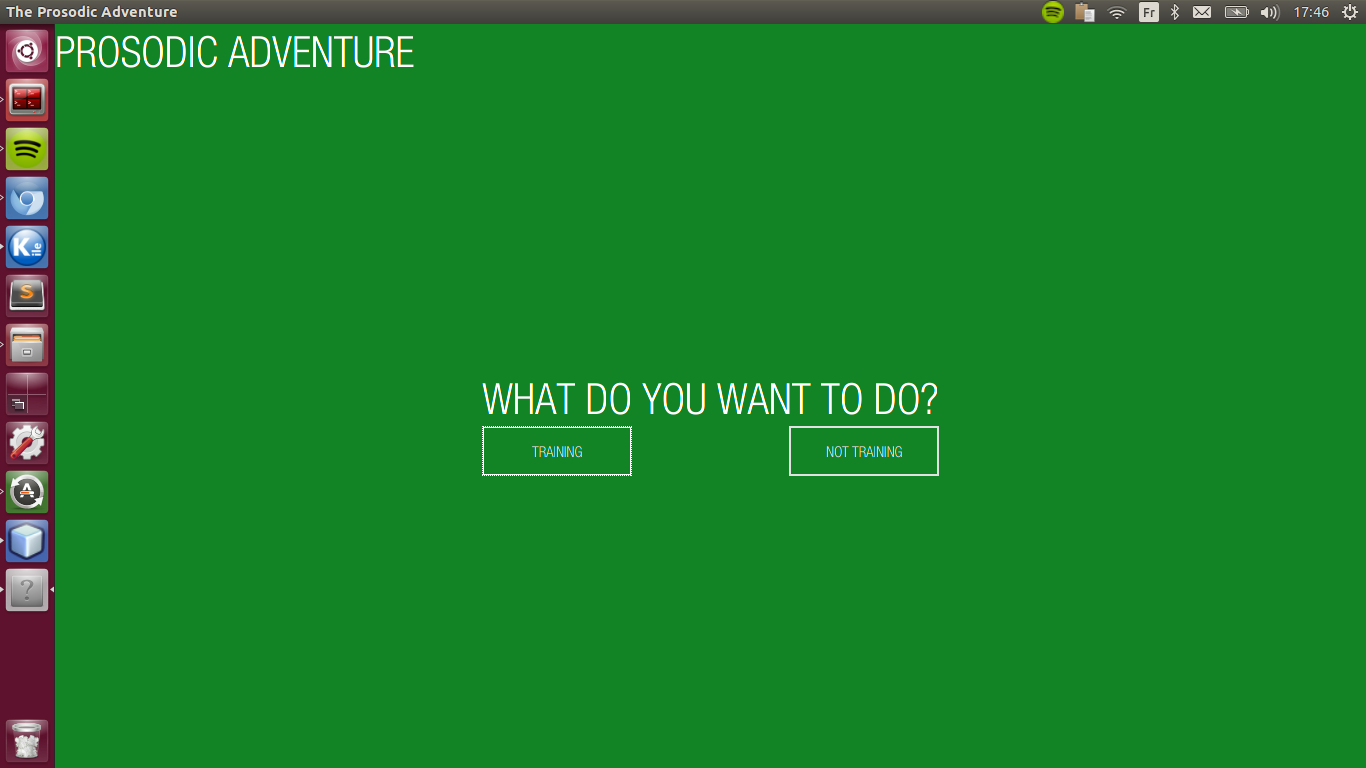
\includegraphics[width=8cm]{./fonctionnement_tests/ChooseGUI.png}}
  \caption{Fonctionnement - ChooseGUI}
  \label{ChooseGUI} 
\end{center}
\end{figure}

On est ensuite dirigé vers le page de test (identique dans le mode ``\textsc{training}'' et ``\textsc{not training}''). La seule différence entre les deux mode est l'exportation de données : dans le test réel, les données sont exportées tandis que dans le mode de découverte, rien n'est exporté.
Les données exportées sont :
\begin{itemize}
 \item Les questions posées
 \item La vidéo réponse
 \item L'audio réponse
\end{itemize}
Ces données sont exportées lors du clic sur le bouton ``\textsc{next}''.

\begin{figure}[!ht]
\begin{center}
  \fbox{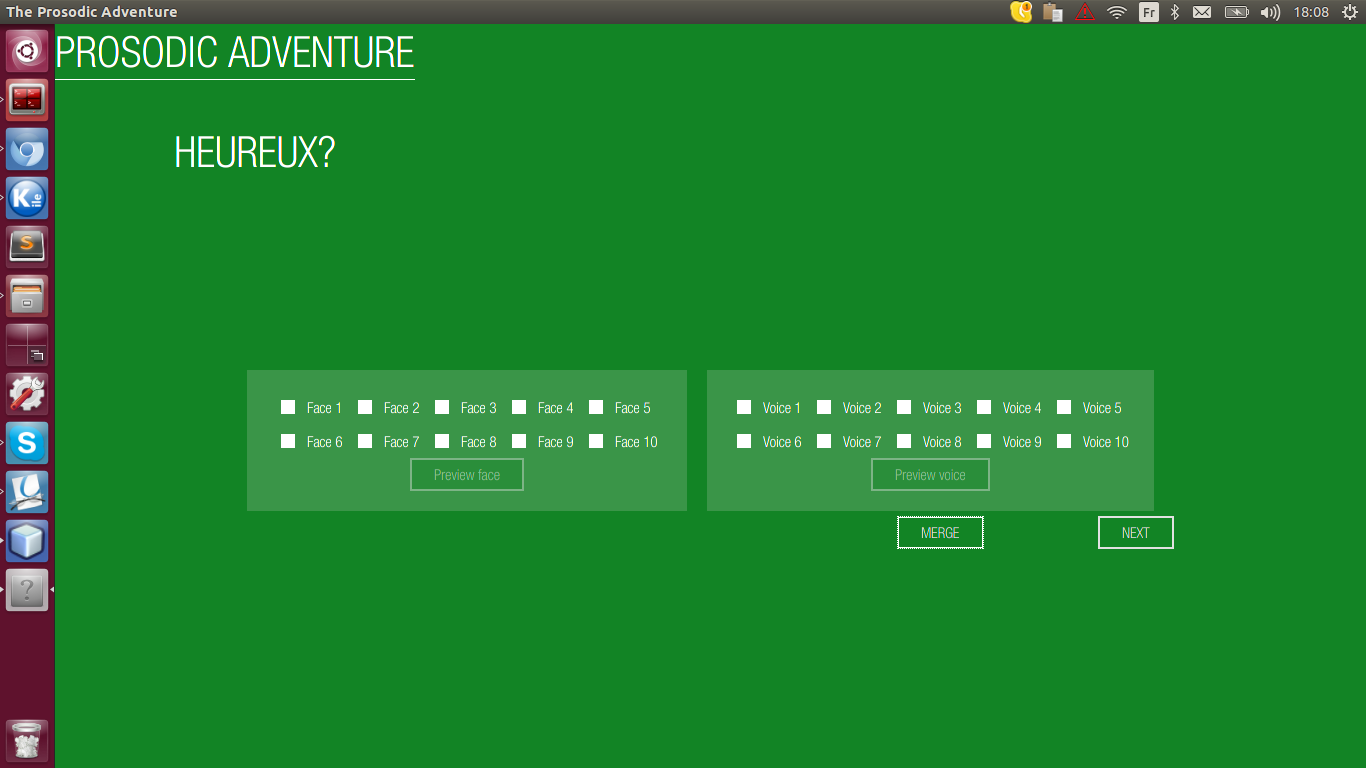
\includegraphics[width=8cm]{./fonctionnement_tests/TestGUI.png}}
  \caption{Fonctionnement - TestGUI}
  \label{ChooseGUI} 
\end{center}
\end{figure}

Les boutons ``\textsc{preview}'' permettent de voir le contenu des vidéos et d'écouter les sons disponibles dans les différentes listes. Afin d'être joués, les médias sont ouverts (voir \textsc{Figure} \ref{VLC} avec VLC (en \textit{standalone}) en faisant appel à la librairie VLC inclue dans le projet.

\begin{figure}[!ht]
\begin{center}
  \fbox{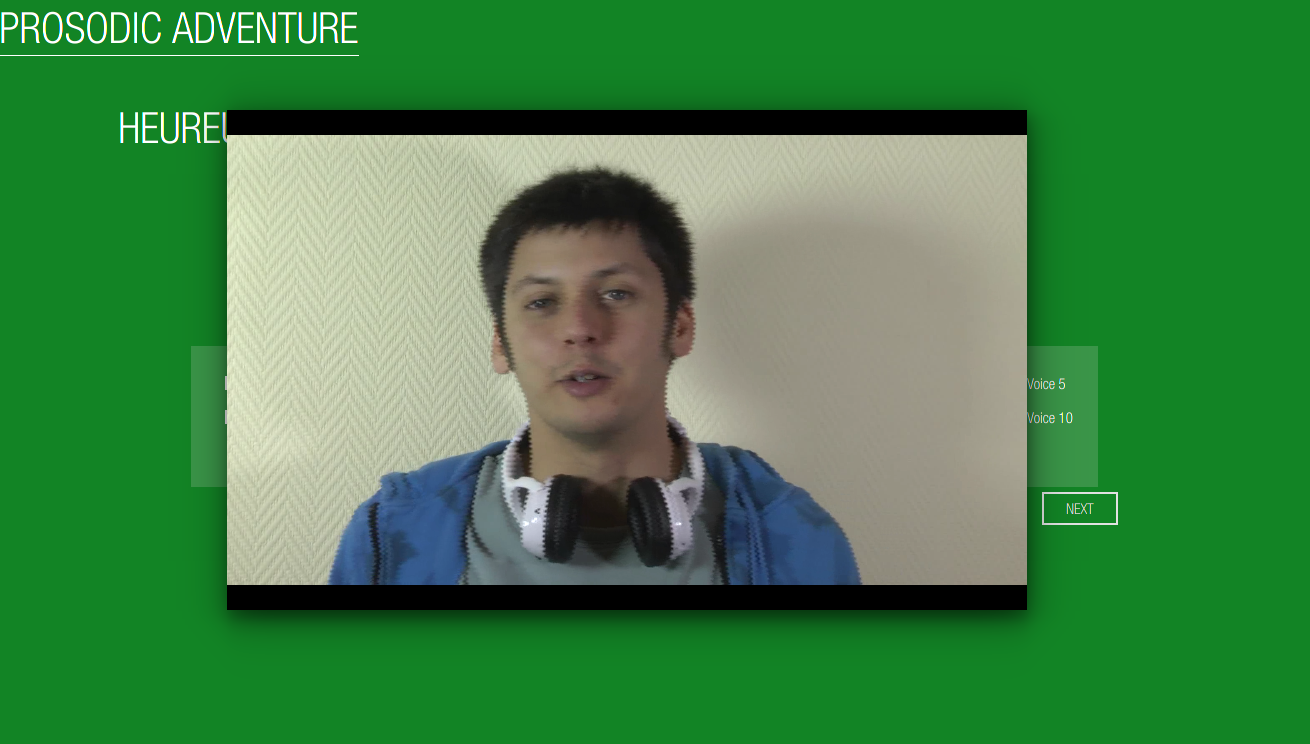
\includegraphics[width=8cm]{./fonctionnement_tests/VLC.png}}
  \caption{Fonctionnement - TestGUI}
  \label{VLC} 
\end{center}
\end{figure}

\subsection{Base de données}

Le système de gestion de base de données relationnelles (SGBDR) choisi a été \textit{SQLite}. Ce SGBDR est utilisable sur n'importe quelle plateforme, sans nécessiter l'installation et la mise en place d'un serveur, il se résume à un fichier \textit{.db} qui contient toute la base de données.
Pour le fontionnement de l'application, différentes fonctions d'accès à la base de données ont été necessaires à implémenter :
\begin{itemize}
 \item Création de la base de données et de ses dépendances (si elle n'existe pas)
 \item Remplissage de la base de données
 \item Consultation du contenu de la base de données
 \item Recherche dans la base de données
 \item Tirage au hasard d'un media de la base de données
 \item Suppression d'un media de la base de données
\end{itemize}
Toutes ces implémentations sont fonctionnelles. Des tests ont été réalisés dessus (voir \ref{tests}).
Les accès à la base de données sont effectués par le driver \textit{Java} de \textit{SQLite} (\textit{sqlite-jdbc-3.8.7}).
Pour éviter tout conflit lors de l'accès à la base de données, des transactions manuelles ont été mises en place : un verrou est créé à chaque accès, ainsi un double accès ne peut pas être effectué.
Etant donné que \textit{SQLite} ne gère pas les contraintes de clef étrangère, nous avons établi un système de vérification en \textit{Java}. Cette vérification vérifie vant chaque modification sensible (suppression d'une vidéo qui pourrait être liée à une question par exemple), qu'aucune dépendance ne sera brisée.


\subsection{Contrôleur}
\lipsum[7]


\subsection{Exportation des données}
\lipsum[8]


\section{Tests}\label{tests}